We show how to control an LED using the M4 on Vaman.
\begin{enumerate}[label=\arabic*.,ref=\theenumi]
\item Check your path
\begin{lstlisting}
cd  vaman/arm/setup/blink/GCC_Project
nvim config.mk
\end{lstlisting}
and
\item and modify so that you have the following lines
\begin{lstlisting}
#export PROJ_ROOT=/data/data/com.termux/files/home/pygmy-dev/pygmy-sdk
export PROJ_ROOT=/root/pygmy-dev/pygmy-sdk
\end{lstlisting}
\item Now execute 
\begin{lstlisting}
cd  vaman/arm/setup/blink/GCC_Project
make -j4
scp  output/bin/blink.bin pi@192.168.0.114:
\end{lstlisting}
Appropriately modify the above ip address before sending blink.bin to the pi.
\item Now log on to the RPi and execute the following
\begin{lstlisting}
sudo python3 /home/pi/Vaman-dev/Vaman-sdk/TinyFPGA-Programmer-Application/tinyfpga-programmer-gui.py --port /dev/ttyACM0  --m4app  blink.bin --mode m4-fpga
\end{lstlisting}
\item Enter the appropriate USB device port above while executing.  Press the button to the right
after the above command is successfully executed.  The LED will start blinking. 
\item See the following lines of the code below
\label{सम:क्रमादेश}
\begin{lstlisting}
codes/setup/blink/src/main.c
\end{lstlisting}
%की  इन पङ्क्तियों पर ध्यान दें । 
%
\begin{lstlisting}
    PyHal_Set_GPIO(18,1);//blue
    PyHal_Set_GPIO(21,1);//green
    PyHal_Set_GPIO(22,1);//red
        HAL_DelayUSec(2000000);
    PyHal_Set_GPIO(18,0);
    PyHal_Set_GPIO(21,0);
    PyHal_Set_GPIO(22,0);
\end{lstlisting}
%
We may conclude that the blink delay is 2000 000us = 2 s.
%इससे हम ज्ञात कर सकते हैं की वामन के दीप का शमीलनकाल 2000 000us = 2 s।  
\item Replace the following line in \ref{सम:क्रमादेश}  
\label{सम:द्विआधार}
\begin{lstlisting}
        HAL_DelayUSec(2000000);
\end{lstlisting}
%
with
\begin{lstlisting}
        HAL_DelayUSec(1000000);
\end{lstlisting}
and execute.  Can you see any difference in the blink period?
%से प्रतिस्थापित कर क्रमादेश का चालयन करें ।  क्या श्मीलनकाल में कोई परिवर्तन द्रश्य है?
\item To obtain red colour, execute the following code.
%रक्तिम रंगोत्पदन के लिए निम्न गूढ़ का चालयन करें।  
\begin{lstlisting}
vaman/arm/codes/setup/red/src/main.c
\end{lstlisting}
Now obtain blue colour.
%इदान हरित एवं नील रंग में दीप को श्मीलित करें।

\item Now obtain green colour without blink.
%इदान  आर्म-जीसीसी  के द्वारा दीप में स्थायी रूप से  हरित वर्ण को उपलब्ध करें।
\\
\solution Execute the following code.
\begin{lstlisting}
vaman/arm/codes/setup/onoff/src/main.c
\end{lstlisting}
%
\item  Using Table  \ref{tab:vaman/arm/setup/input} and 
\figref{fig:vaman-pin_sheet},
 use an input pin to control the onboard LED.  
%एक अन्य कुश को निर्गत रूप देकर किसी बाह्य दीप को प्रकाशोर्जित करें.

\begin{table}[]
\centering
\begin{tabular}{|l|l|l|}
\hline
Type & Pin  &  Destination\\ \hline
Input &  IO\_5 &  5V\\ \hline
%आगत &  IO\_28 &  GND\\ \hline
%निर्गत  & IO\_11  &  LED\\ \hline
\end{tabular}
\caption{Vaman control through external input.}
\label{tab:vaman/arm/setup/input}
\end{table}
\iffalse
\begin{figure*}[!ht]
\centering
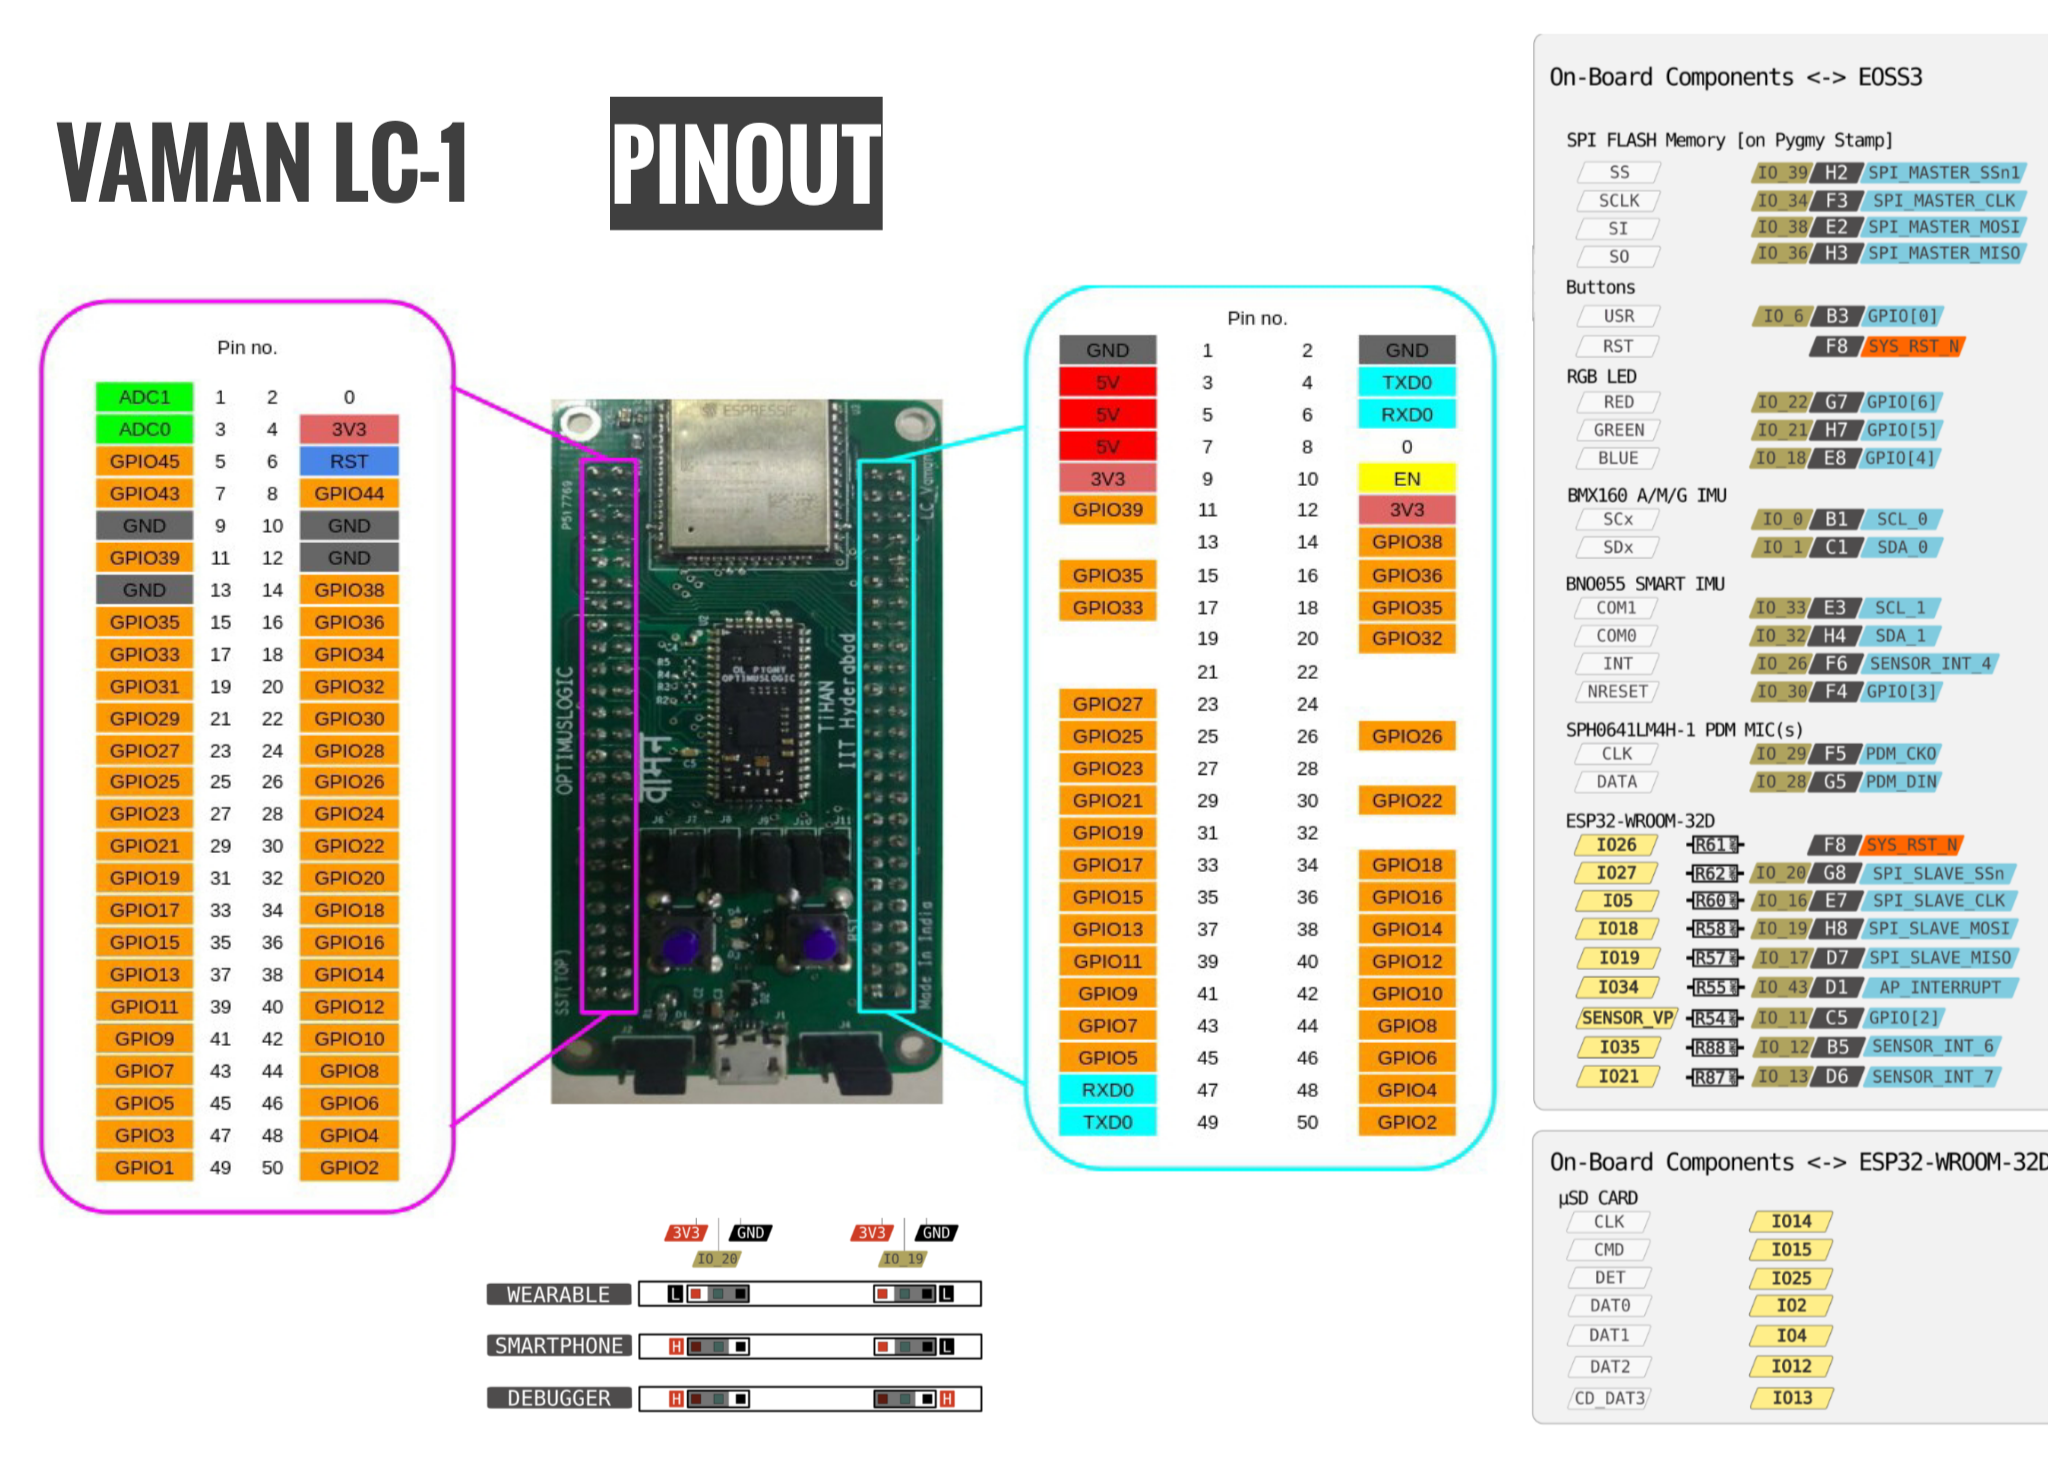
\includegraphics[width = \textwidth]{vaman/arm/setup/figs/pin_sheet.png}
\caption{Pin Diagram}
\label{fig:vaman/arm/setup/pin_sheet}
\end{figure*}
\fi
\solution Execute the following code.  You should see the green LED on.   Connecting IO\_5 to GND will turn the green LED off.
\begin{lstlisting}
vaman/arm/codes/setup/gpio/src/main.c
\end{lstlisting}
\item Execute the codes in 
\begin{lstlisting}
vaman/arm/codes/sevenseg/loop/
\end{lstlisting}
to control the seven segment display.

\end{enumerate}


